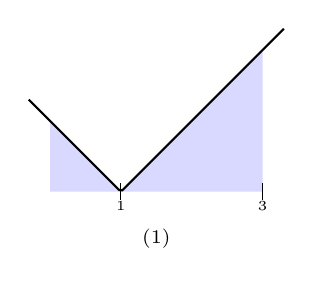
\begin{tikzpicture}[x=9mm,y=9mm]
\fill[blue!15] (0,1)--(1,0)--(3,2)--(3,0)--(0,0)--cycle;
\ax{-0.5}{3.5}{-0.5}{2.6}
\draw[thick,domain=-0.3:3.3,samples=80] plot (\x,{abs(\x-1)});
\draw (1,0.12)--(1,-0.12); \node[below] at (1,0){\tiny $1$};
\draw (3,0.12)--(3,-0.12); \node[below] at (3,0){\tiny $3$};
\node[below] at (current bounding box.south){\scriptsize (1)};
\end{tikzpicture}